\documentclass{exam}
\setlength{\parskip}{0pt}
\setlength{\parindent}{0pt}
\setlength{\voffset}{-15pt}
\usepackage[onehalfspacing]{setspace} % Sets Spacing to 1.5
\usepackage[utf8]{inputenc} % Use UTF-8 encoding
\usepackage{float} % Improved interface for floating objects
\usepackage[colorlinks = true,
            linkcolor = blue,
            urlcolor  = blue,
            citecolor = blue,
            anchorcolor = blue]{hyperref} % For hyperlinks in the PDF
\usepackage{graphicx, multicol} % Enhanced support for graphics
\usepackage{amsmath}
\usepackage{framed, caption}
\usepackage{array}
\usepackage{float}
\usepackage{amsmath}
\usepackage{bbm}
\newcommand\tab[1][0.2cm]{\hspace*{#1}}
\usepackage{multicol}
%----------------------------------------------------------------------------------------
\begin{document}

\begin{minipage}{0.295\textwidth} % Left side of title section
\raggedright
COL362 - Intro. to DBMS\\ % Your lecture or course
\footnotesize % Authors text size
CSE, IIT Delhi (SEM2, 2020-21) % Department
\medskip\hrule
\end{minipage}
\begin{minipage}{0.4\textwidth} % Center of title section
\centering 
\large % Title text size
\textbf{Assignment 1}\\ % Assignment number
\normalsize % Subtitle text size
 % Assignment subtitle
\end{minipage}
\begin{minipage}{0.295\textwidth} % Right side of title section
\raggedleft
2018CS10388\\ % Entry Number
\footnotesize
Sharique Shamim % Name
\medskip\hrule
\end{minipage}
\vspace{0.1in}
\section{Time taken for each query}
\begin{figure}[h]
\centering
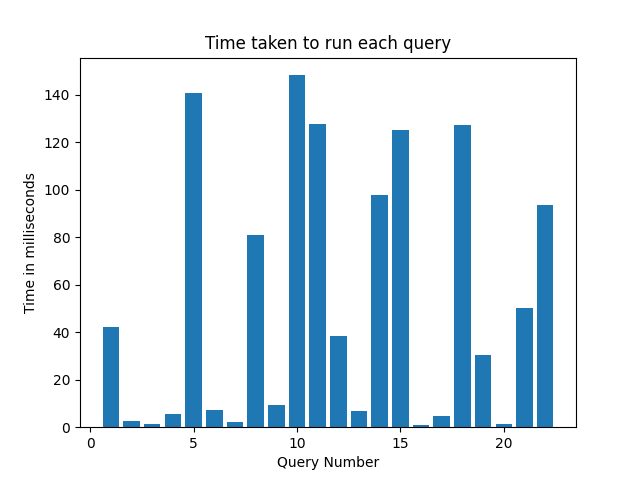
\includegraphics[scale=1.0]{query.png}
\end{figure}
\begin{center}
\begin{tabular}{ | p{5cm} | p{5cm} |  }
\hline \centering \textbf{Query Number } & \textbf{Time in milliseconds} \\
\hline \centering \texttt{$1$} &  42.159 ms\\
\hline \centering \texttt{$2$} &  2.772 ms\\
\hline \centering \texttt{$3$} &  1.356 ms\\
\hline \centering \texttt{$4$} &  5.583 ms\\
\hline \centering \texttt{$5$} &  140.532 ms\\
\hline \centering \texttt{$6$} &  7.282 ms\\
\hline \centering \texttt{$7$} &  2.090 ms\\
\hline \centering \texttt{$8$} &  80.757 ms\\
\hline \centering \texttt{$9$} & 9.172 ms\\
\hline \centering \texttt{$10$} & 127.708 ms\\
\hline \centering \texttt{$11$} &  38.419 ms\\
\hline \centering \texttt{$12$} & 71.749 ms\\
\hline \centering \texttt{$13$} & 6.919 ms\\
\hline \centering \texttt{$14$} &  97.546 ms\\
\hline \centering \texttt{$15$} & 125.050 ms\\
\hline \centering \texttt{$16$} & 0.806 ms\\
\hline \centering \texttt{$17$} & 4.865 ms\\
\hline \centering \texttt{$18$} & 127.150 ms\\
\hline \centering \texttt{$19$} & 30.470 ms\\
\hline \centering \texttt{$20$} &  1.306 ms\\
\hline \centering \texttt{$21$} & 50.226 ms\\
\hline \centering \texttt{$22$} & 93.507 ms \\
\hline
\end{tabular}
\end{center}
\end{document}